\section{Clients SIP}

Afin de tester le bon fonctionnement des serveurs et de remplir les journaux, nous avons dû utiliser des clients SIP. Nous avons principalement utilisé les clients logiciels, mais nous avons aussi essayé des clients matériels.

\subsection{\xlite}

\begin{figure}[h]
\begin{center}
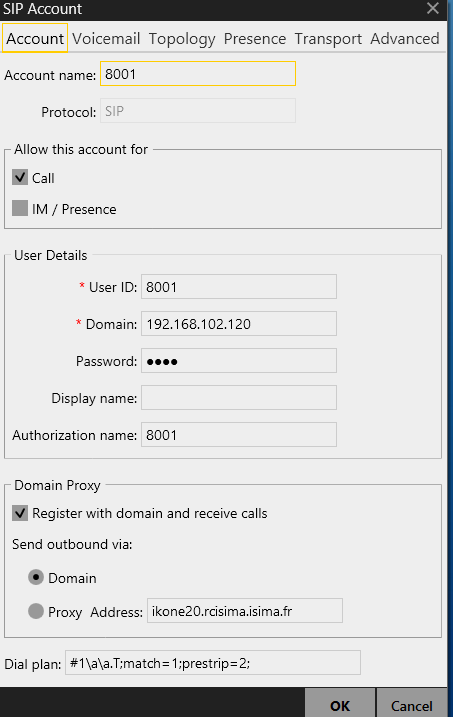
\includegraphics[width=7cm]{images/config-xlite.png}
\end{center}
\caption{Panneau de configuration de Xlite}
\end{figure}

Suite à la rapide présentation qui nous en avait été faite en cours de téléphonie, nous avons commencé par utiliser {\xlite}. {\xlite} est un client SIP logiciel développé par la société CounterPath. Il est disponible pour {\win} et {\mac}. Le fait qu’il ne soit plus disponible pour {\lnx} nous a amenés à peu l’utiliser, afin de simplifier notre organisation.

\todo[Expliquer brièvement la configuration]

\subsection{\lnp}

\begin{figure}[h]
\begin{center}
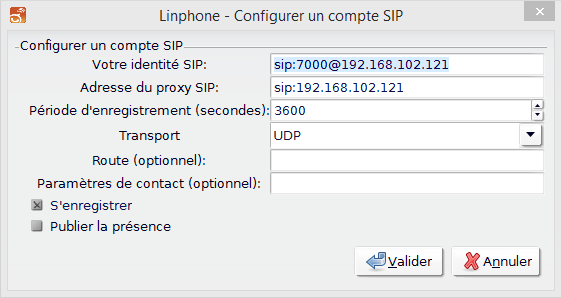
\includegraphics[width=12cm]{images/config-linphone.png}
\end{center}
\caption{Panneau de configuration de Linphone}
\end{figure}

Nous avons donc recherché un client logiciel disponible pour {\lnx} ; après avoir testé plusieurs logiciels non fonctionnels à cause d’erreurs de compilation, dues à des incompatibilité avec des bibliothèques trop récentes, et d’erreurs de segmentation à l’exécution, nous avons trouvé {\lnp}, qui fonctionne bien et qui a l’avantage d’être disponible dans les dépôts de la plupart des distributions {\lnx}.

\todo[Étoffer un peu la description ?]

{\lnp} est un logiciel \textit{open source} disponible pour les principaux systèmes d’exploitation, aussi bien bureau que mobile.

\todo[Expliquer brièvement la configuration]

\subsection{\cph}

\begin{figure}[h]
\begin{center}
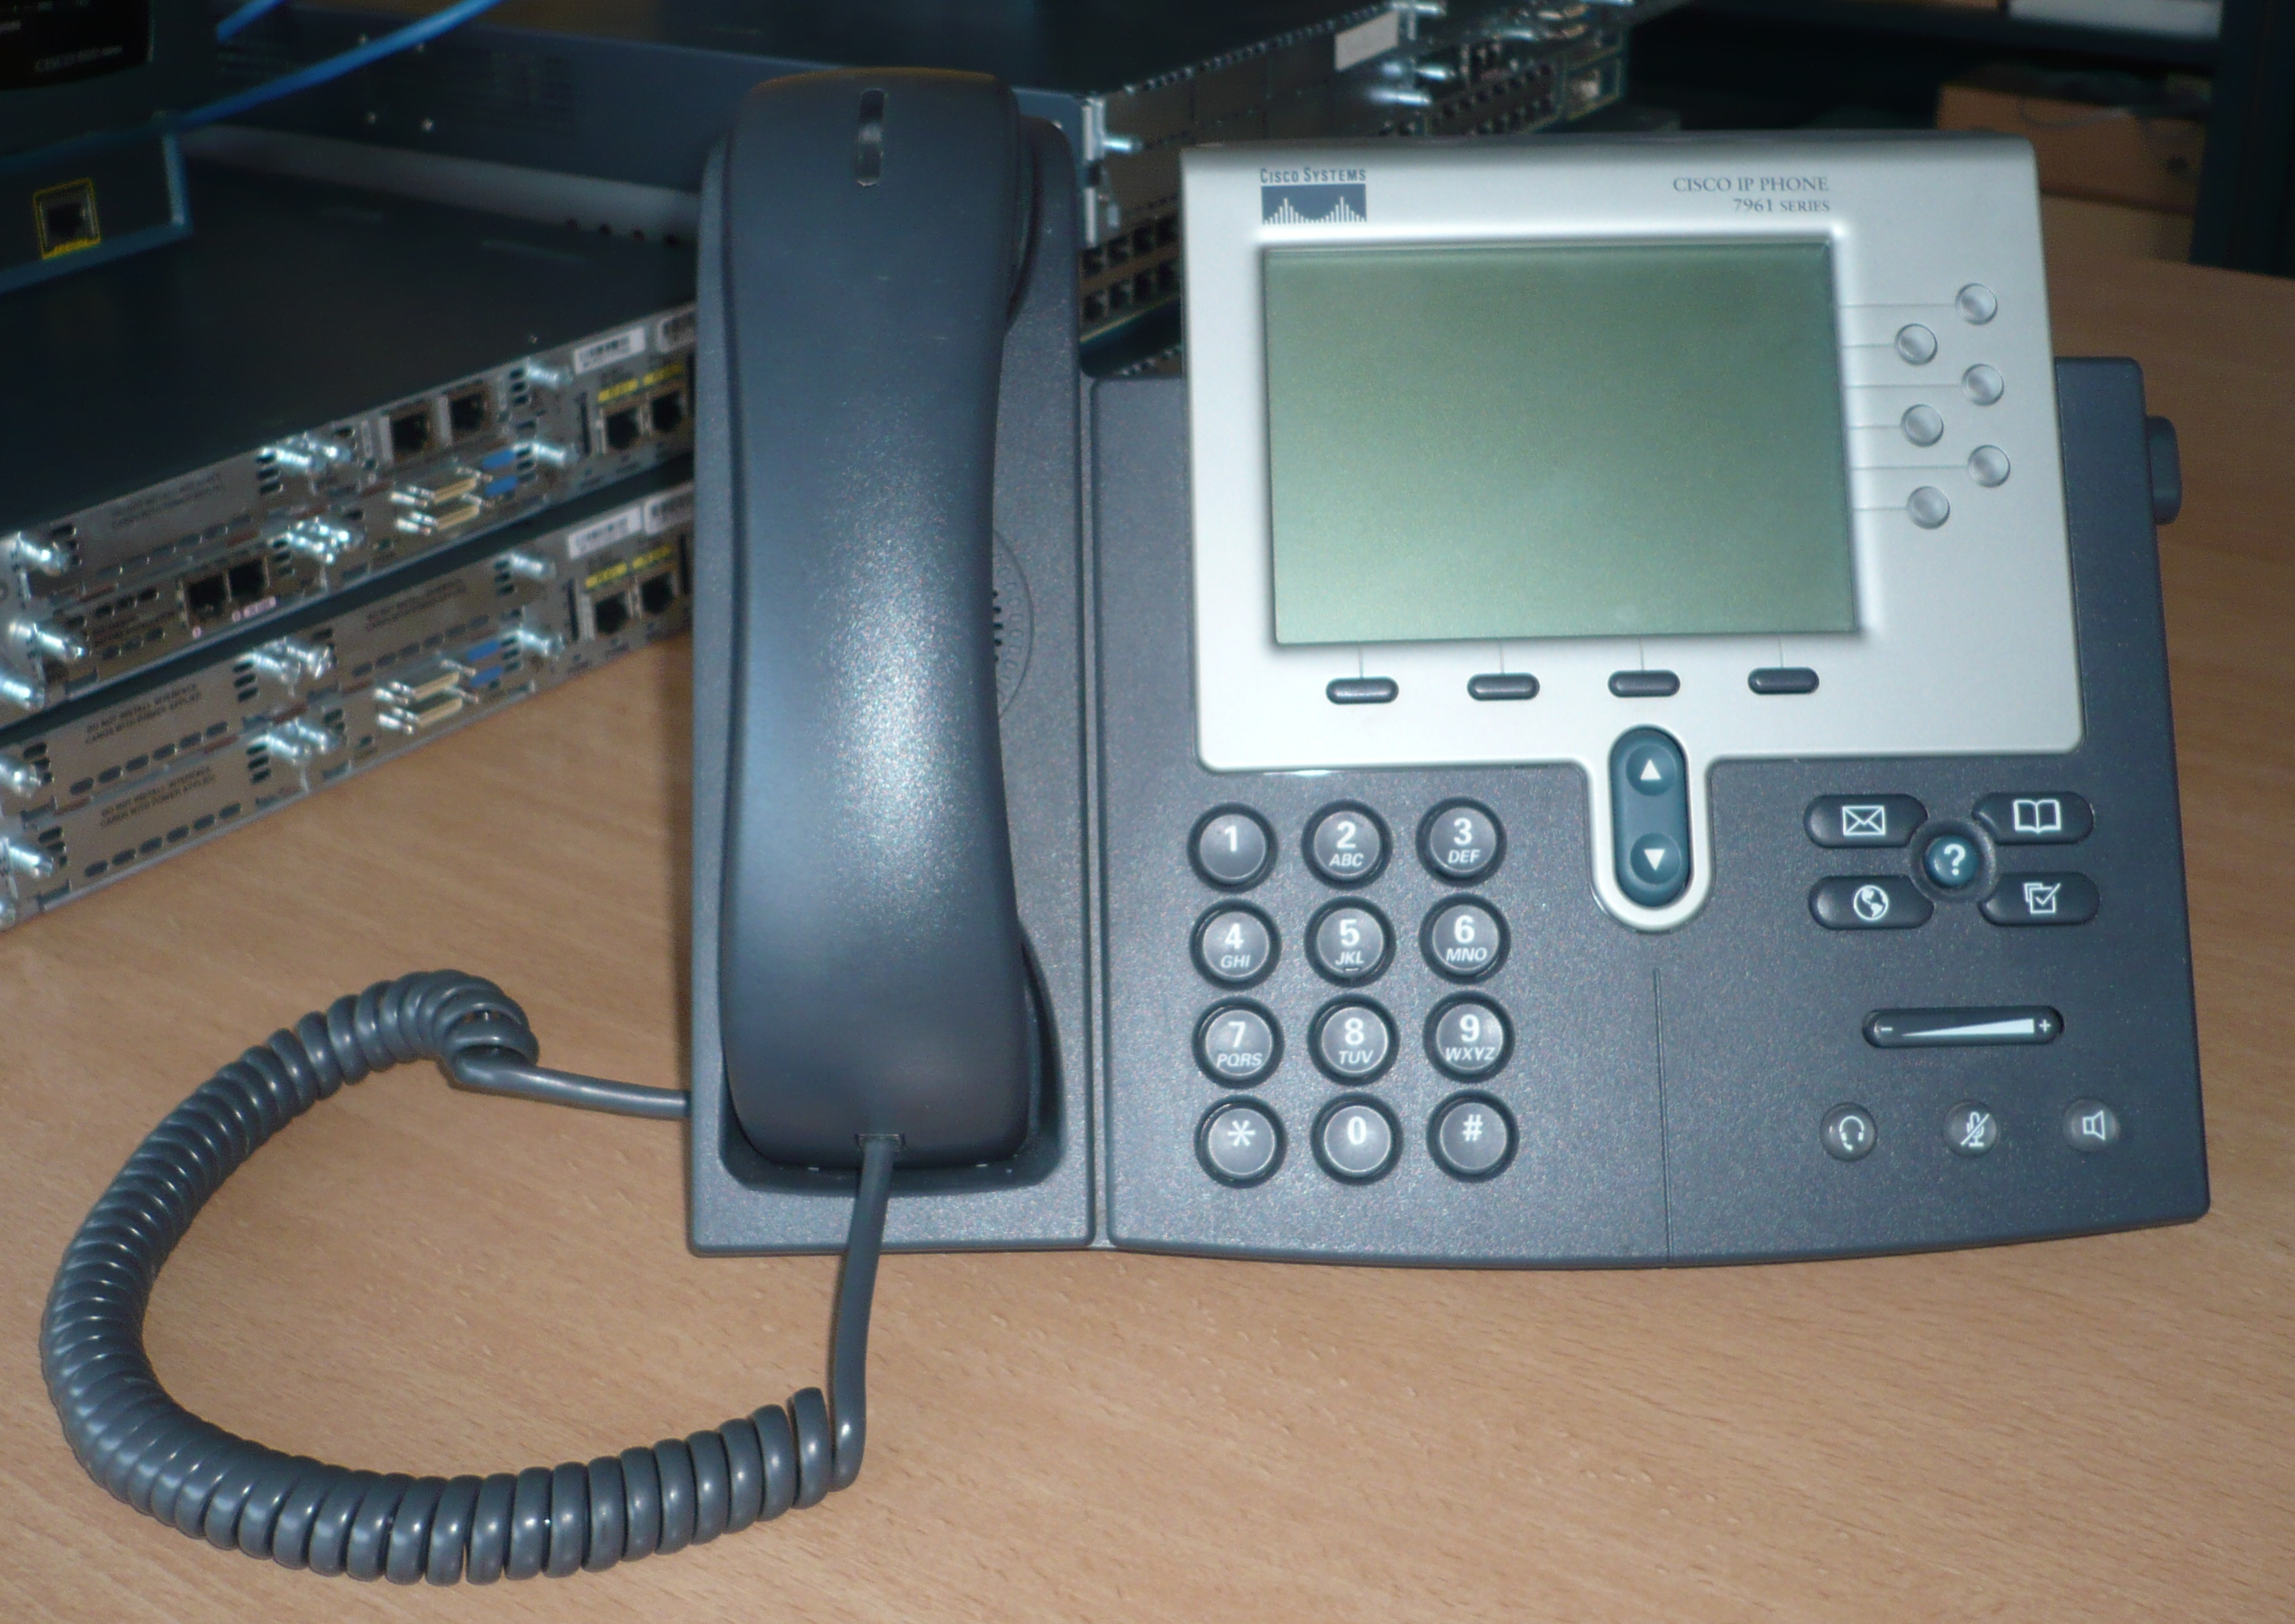
\includegraphics[width=7cm]{images/7961.jpg}
\end{center}
\caption{\cph}
\end{figure}

Le {\cph} est un téléphone fonctionnant en VoIP vendu par Cisco. Nous avons tenté d'utiliser un {\cph} dans le cadre de notre projet. Pour cela, il a fallu installer un serveur TFTP afin de permettre au téléphone de trouver sa configuration.
Nous avons néanmoins rapidement rencontré des problèmes avec cette configuration.
C'est pourquoi nous avons décidé d'utiliser plutôt un {\ata}. 
\todo[Problème des mots de passe]

\subsection{\cata}

\begin{figure}[h]
\begin{center}
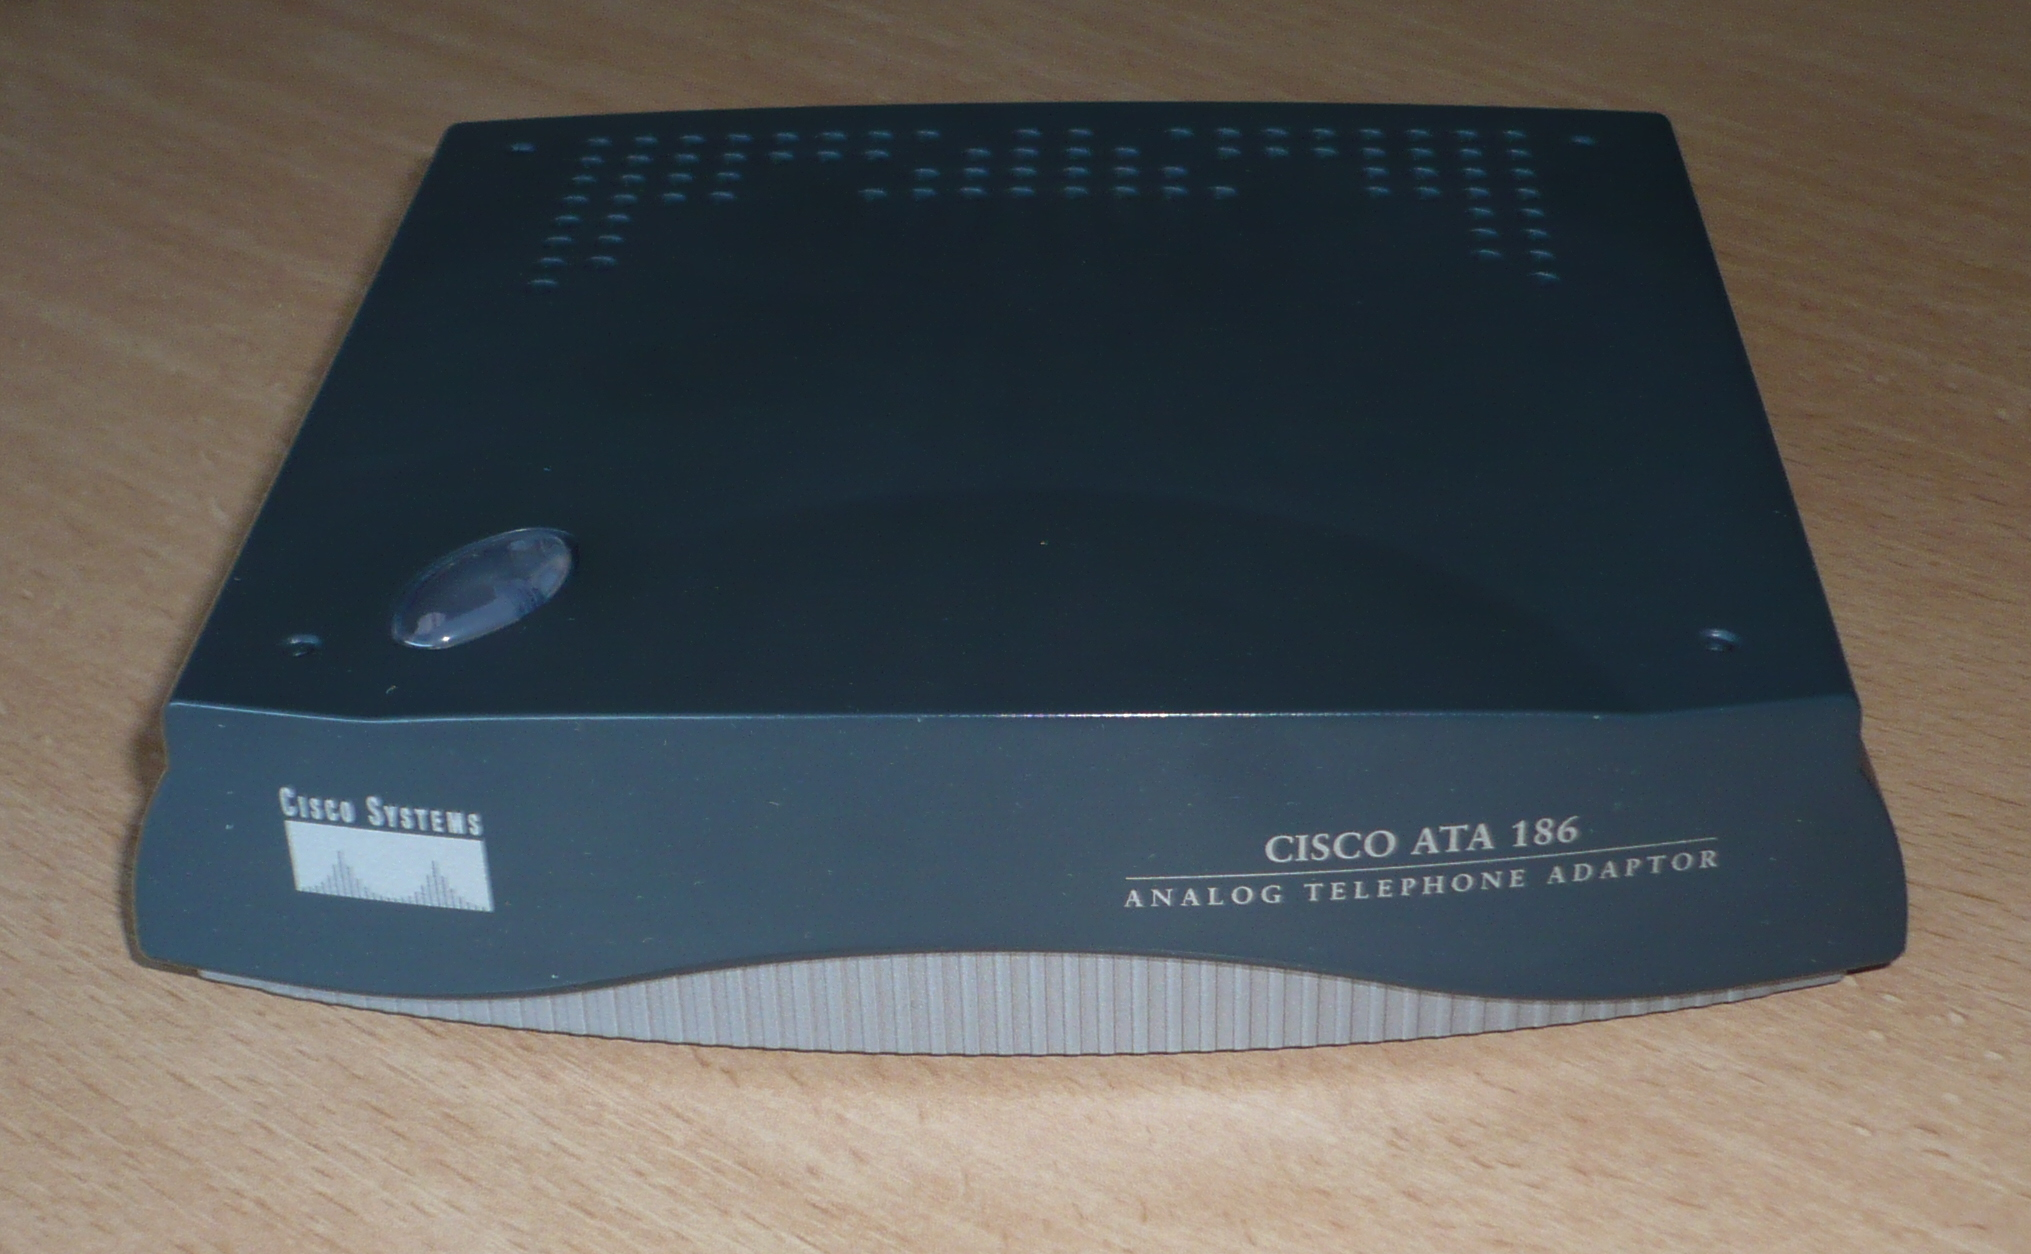
\includegraphics[width=7cm]{images/ata.jpg}
\end{center}
\caption{\ata}
\end{figure}

Un {\ata} (Analog Telephone Adaptor) est un adaptateur combiné à Ethernet permettant de faire fonctionner un téléphone analogique en VoIP.

\todo[Description de la configuration ; problème de la résolution de nom]
